% Options for packages loaded elsewhere
\PassOptionsToPackage{unicode}{hyperref}
\PassOptionsToPackage{hyphens}{url}
%
\documentclass[
]{article}
\usepackage{amsmath,amssymb}
\usepackage{lmodern}
\usepackage{ifxetex,ifluatex}
\ifnum 0\ifxetex 1\fi\ifluatex 1\fi=0 % if pdftex
  \usepackage[T1]{fontenc}
  \usepackage[utf8]{inputenc}
  \usepackage{textcomp} % provide euro and other symbols
\else % if luatex or xetex
  \usepackage{unicode-math}
  \defaultfontfeatures{Scale=MatchLowercase}
  \defaultfontfeatures[\rmfamily]{Ligatures=TeX,Scale=1}
\fi
% Use upquote if available, for straight quotes in verbatim environments
\IfFileExists{upquote.sty}{\usepackage{upquote}}{}
\IfFileExists{microtype.sty}{% use microtype if available
  \usepackage[]{microtype}
  \UseMicrotypeSet[protrusion]{basicmath} % disable protrusion for tt fonts
}{}
\makeatletter
\@ifundefined{KOMAClassName}{% if non-KOMA class
  \IfFileExists{parskip.sty}{%
    \usepackage{parskip}
  }{% else
    \setlength{\parindent}{0pt}
    \setlength{\parskip}{6pt plus 2pt minus 1pt}}
}{% if KOMA class
  \KOMAoptions{parskip=half}}
\makeatother
\usepackage{xcolor}
\IfFileExists{xurl.sty}{\usepackage{xurl}}{} % add URL line breaks if available
\IfFileExists{bookmark.sty}{\usepackage{bookmark}}{\usepackage{hyperref}}
\hypersetup{
  pdftitle={Astrostatistics \& Cosmology, ex. 1},
  pdfauthor={Marco Giunta},
  hidelinks,
  pdfcreator={LaTeX via pandoc}}
\urlstyle{same} % disable monospaced font for URLs
\usepackage[margin=1in]{geometry}
\usepackage{graphicx}
\makeatletter
\def\maxwidth{\ifdim\Gin@nat@width>\linewidth\linewidth\else\Gin@nat@width\fi}
\def\maxheight{\ifdim\Gin@nat@height>\textheight\textheight\else\Gin@nat@height\fi}
\makeatother
% Scale images if necessary, so that they will not overflow the page
% margins by default, and it is still possible to overwrite the defaults
% using explicit options in \includegraphics[width, height, ...]{}
\setkeys{Gin}{width=\maxwidth,height=\maxheight,keepaspectratio}
% Set default figure placement to htbp
\makeatletter
\def\fps@figure{htbp}
\makeatother
\setlength{\emergencystretch}{3em} % prevent overfull lines
\providecommand{\tightlist}{%
  \setlength{\itemsep}{0pt}\setlength{\parskip}{0pt}}
\setcounter{secnumdepth}{-\maxdimen} % remove section numbering
\ifluatex
  \usepackage{selnolig}  % disable illegal ligatures
\fi

\title{Astrostatistics \& Cosmology, ex. 1}
\author{Marco Giunta}
\date{21/10/2021}

\begin{document}
\maketitle

\hypertarget{introduction}{%
\section{Introduction}\label{introduction}}

In order to solve the exercise we need to perform a straightforward
application of Bayes' theorem; since this is a one dimensional problem
(in the sense that we only need to infer one parameter) there will be no
need for special techniques, such as Markov chains.

Let's then setup the mathematics of the problem of inferring the coin
bias as follows. We model the process of obtaining heads/tails when we
toss a coin \(N\) times as a \emph{binomial process}, in the sense that
if the probability of obtaining e.g.~heads is equal to \(H\) then the
probability distribution of obtaining \(n\) heads in \(N\) tosses is
given by the \emph{binomial distribution}: \begin{equation}
  p(n,N|H) \propto H^n (1-H)^{N-n}
\end{equation} where the proportionality constant is the binomial
coefficient of \(n\) over \(N\), which we don't need to write explicitly
here since we will simply normalize the final posterior distribution.

Notice that by using this pdf as our likelihood function we can easily
simulate coin tosses once we specify the value of \(H\); if instead
\(H\) is unknown we need to perform an \emph{inference} according to
some rule. The frequentist prescription for this problem is to feed the
experimental values of \(n\) and \(N\), then treat the result as a
function of \(H\) and maximize it (MLE paradigm).\\
The bayesian approach, instead, is to multiply the likelihood by an
arbitrarily chosen prior, then normalize the result to obtain the
posterior (which naturally encodes the idea of leftover uncertainty over
\(H\) due to the finiteness of the available dataset).

This means that in order to solve the exercise we must first multiply
the binomial likelihood (where \(n\) and \(N\) are fixed, and \(H\) is a
random variable) by either the uniform or the gaussian prior, then
normalize the result to obtain the posterior.\\
Mathematically speaking we write: \begin{equation}
  P(H|n,N) = \frac{P(n,N|H)P(H)}{\int_0^1 P(n,N|H)P(H) \ \mathrm{d}H}
\end{equation} which is nothing else than Bayes' theorem applied to the
specific problem at hand.

Notice that the posterior distribution will be a 1D pdf defined over the
\([0,1]\) interval, as its only argument is the probability of obtaining
heads in a single toss; this means that we can easily normalize it, for
example by approximating the evidence integral as a Riemann sum:
\begin{equation}
  \int_0^1 P(n,N|H)P(H) \ \mathrm{d}H \approx \sum_i P(n,N|H_i)P(H_i) \Delta H_i
\end{equation} where of course any other numerical scheme is a suitable
alternative.

This technique is quite general, too; it applies to an arbitrary prior,
something which isn't true e.g.~if we use the conjugate prior technique.

\hypertarget{uniform-prior}{%
\section{Uniform prior}\label{uniform-prior}}

Let's start by fixing \(H_{\text{true}} = 0.3\); this allows us to
simulate the experimental data which one would need to collect in order
to perform an ``in real life'' inference.\\
For example the first 10 obtained tosses may be:

\begin{verbatim}
##  [1] "H" "T" "T" "T" "T" "T" "H" "H" "T" "T"
\end{verbatim}

Now we can multiply the binomial likelihood by our prior, then normalize
and plot the result; notice that since a uniform prior is simply a
constant it suffices to normalize the likelihood itself.\\
We plot the posteriors directly because the prior is simply the
\(f(H) = 1\) flat (therefore boring) function.

\begin{center}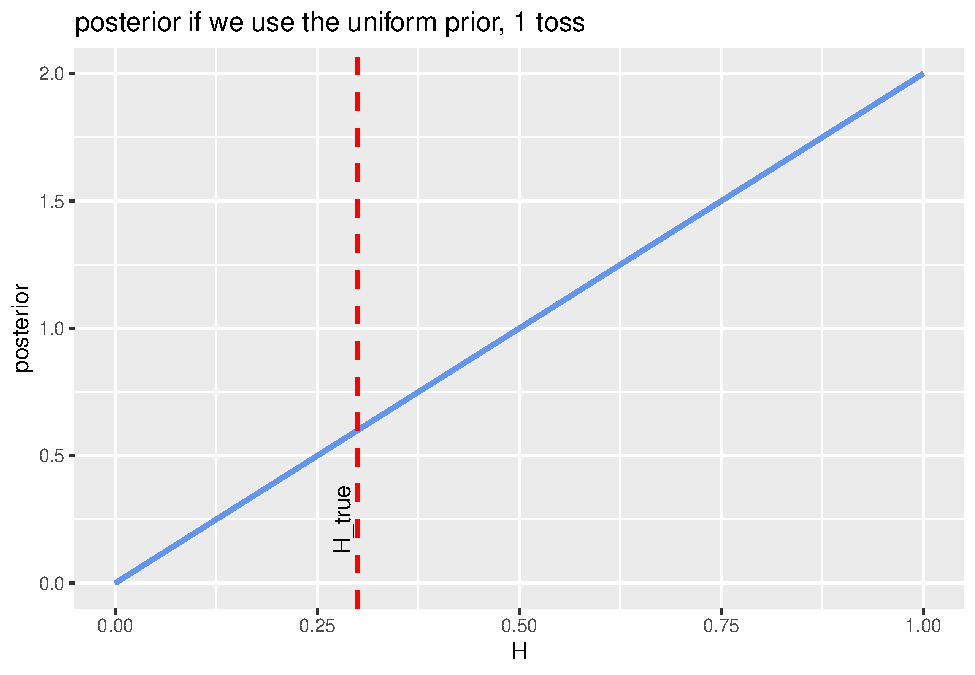
\includegraphics[width=0.75\linewidth]{astrostat-1_files/figure-latex/unnamed-chunk-3-1} \end{center}

\begin{center}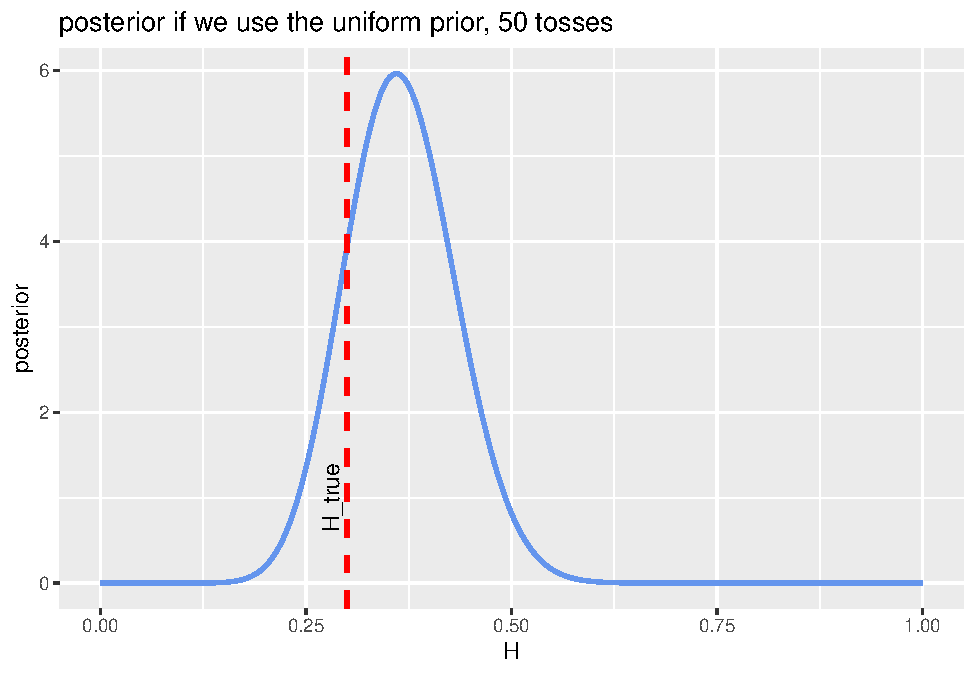
\includegraphics[width=0.75\linewidth]{astrostat-1_files/figure-latex/unnamed-chunk-4-1} \end{center}

\begin{center}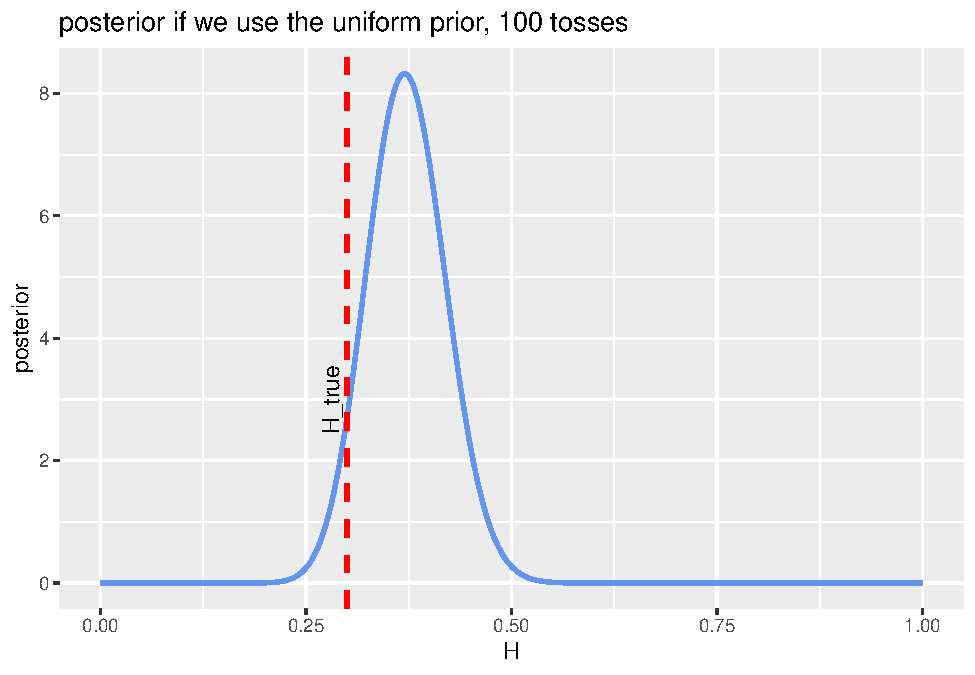
\includegraphics[width=0.75\linewidth]{astrostat-1_files/figure-latex/unnamed-chunk-5-1} \end{center}

\begin{center}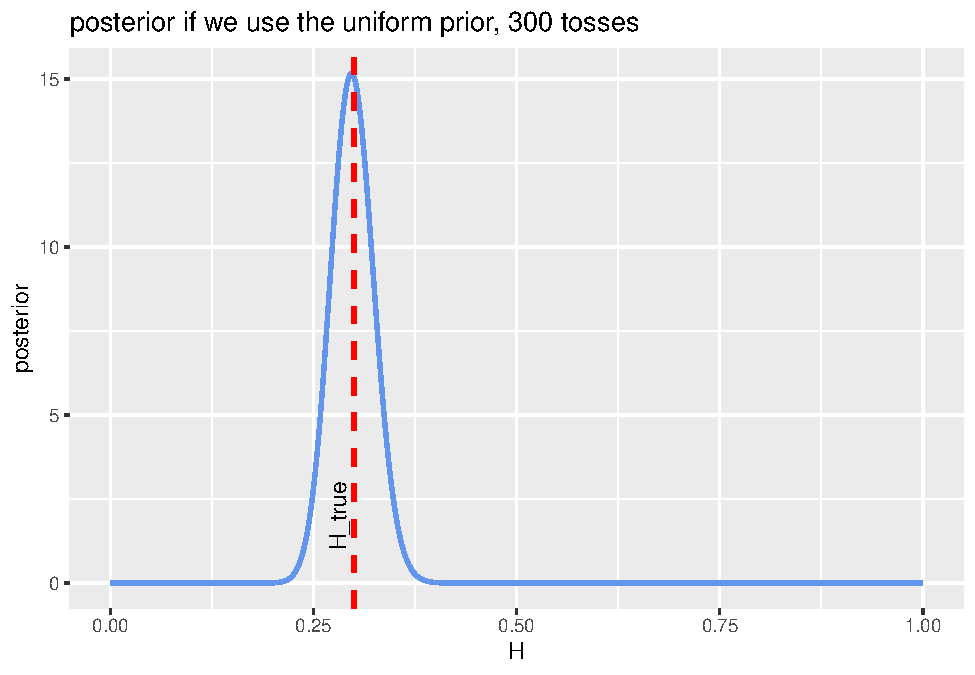
\includegraphics[width=0.75\linewidth]{astrostat-1_files/figure-latex/unnamed-chunk-6-1} \end{center}

\begin{center}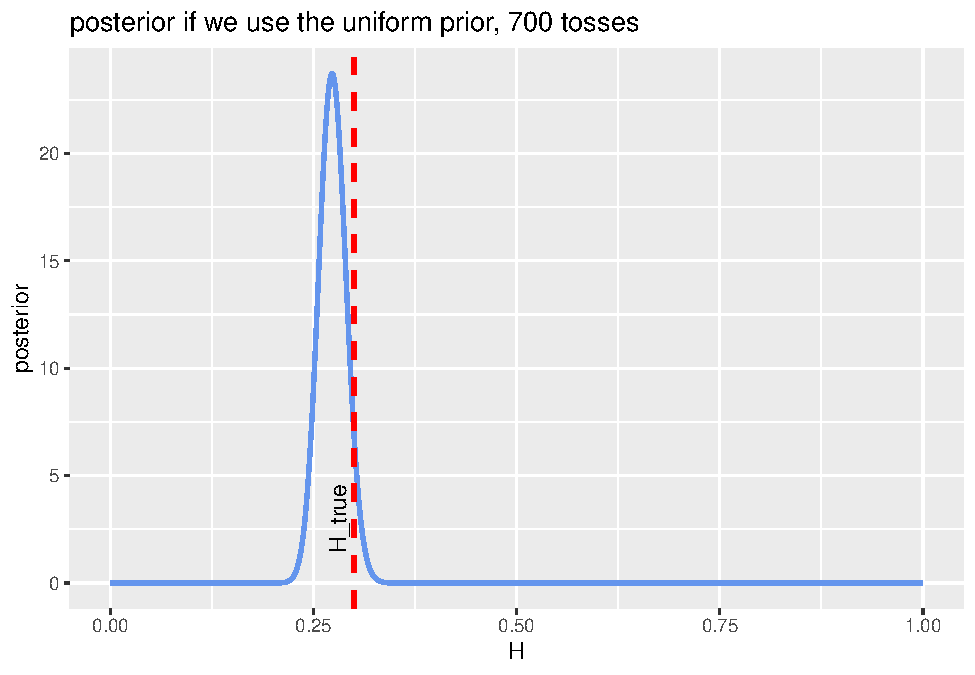
\includegraphics[width=0.75\linewidth]{astrostat-1_files/figure-latex/unnamed-chunk-7-1} \end{center}

\begin{center}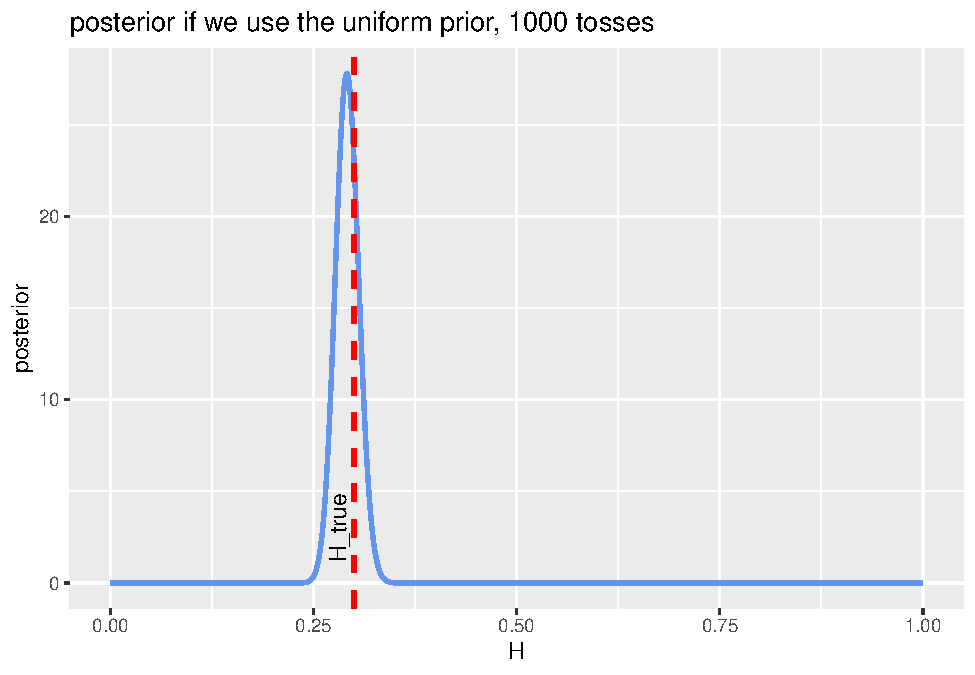
\includegraphics[width=0.75\linewidth]{astrostat-1_files/figure-latex/unnamed-chunk-8-1} \end{center}

Notice that the more data we use the more satisfying the resulting
posterior is. Indeed when we use more data the posterior's center
becomes closer to the true value (which means we're getting closer and
closer to the ``correct'' value), while at the same time the posterior
itself becomes narrower (which means that the uncertainty with which we
inferred \(H\) is decreasing, as it should).\\
As we know we can be confident that in the \(N \to + \infty\) limit we
will obtain \(H_{\text{true}}\), and yet when the dataset is still small
the posterior isn't very good (cfr the \(N=1\) plot above). One may
wonder whether a smarter choice of the prior may accelerate the
convergence; indeed this is exactly what we want to check in the next
part of the exercise.

\hypertarget{gaussian-prior}{%
\section{Gaussian prior}\label{gaussian-prior}}

Let us now use a gaussian prior with \(\mu = 0.5\), \(\sigma = 0.1\):

\begin{center}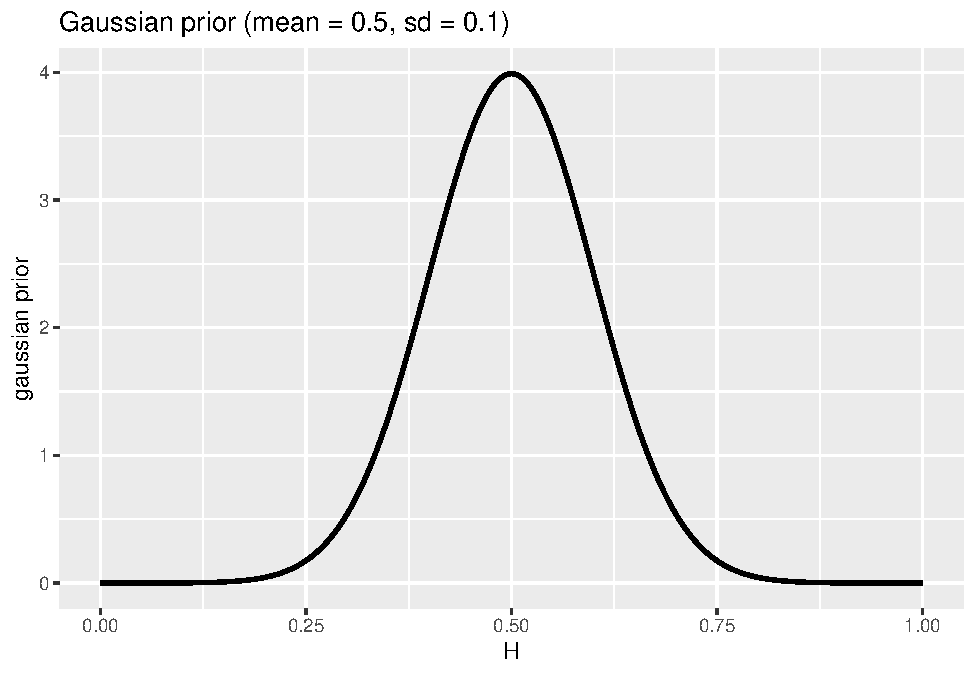
\includegraphics[width=0.75\linewidth]{astrostat-1_files/figure-latex/unnamed-chunk-9-1} \end{center}

To obtain the posterior we multiply this function by the same binomial
likelihood, then normalize the result.

\begin{center}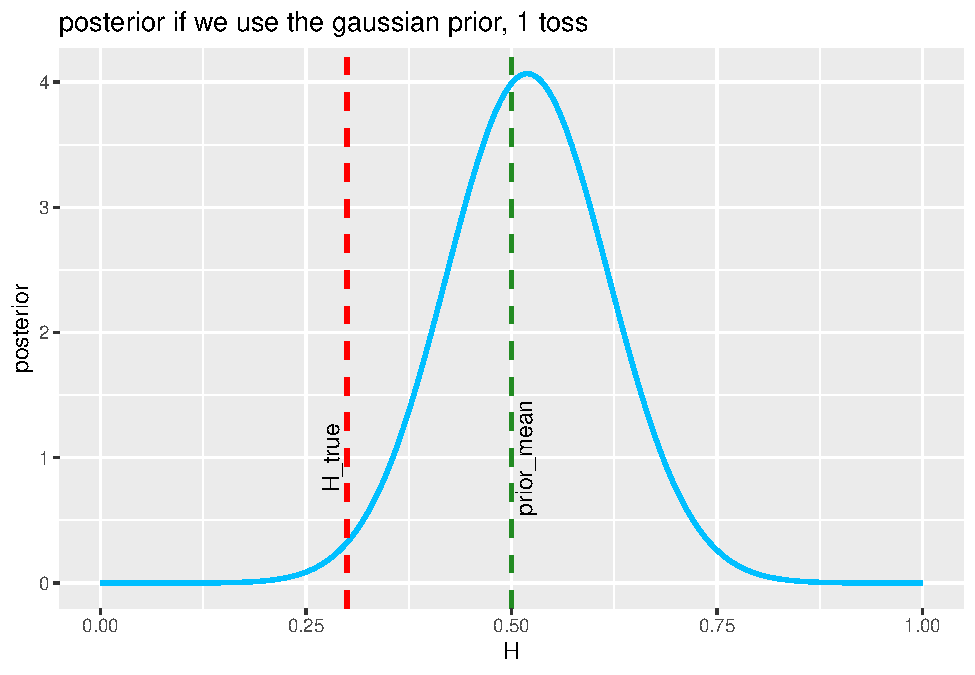
\includegraphics[width=0.75\linewidth]{astrostat-1_files/figure-latex/unnamed-chunk-11-1} \end{center}

\begin{center}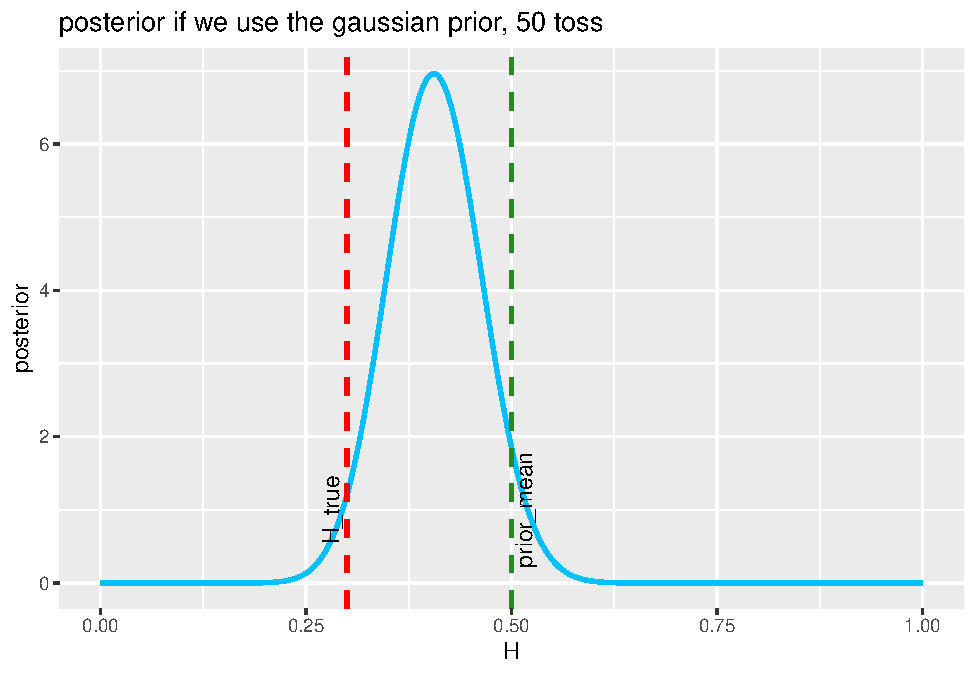
\includegraphics[width=0.75\linewidth]{astrostat-1_files/figure-latex/unnamed-chunk-12-1} \end{center}

\begin{center}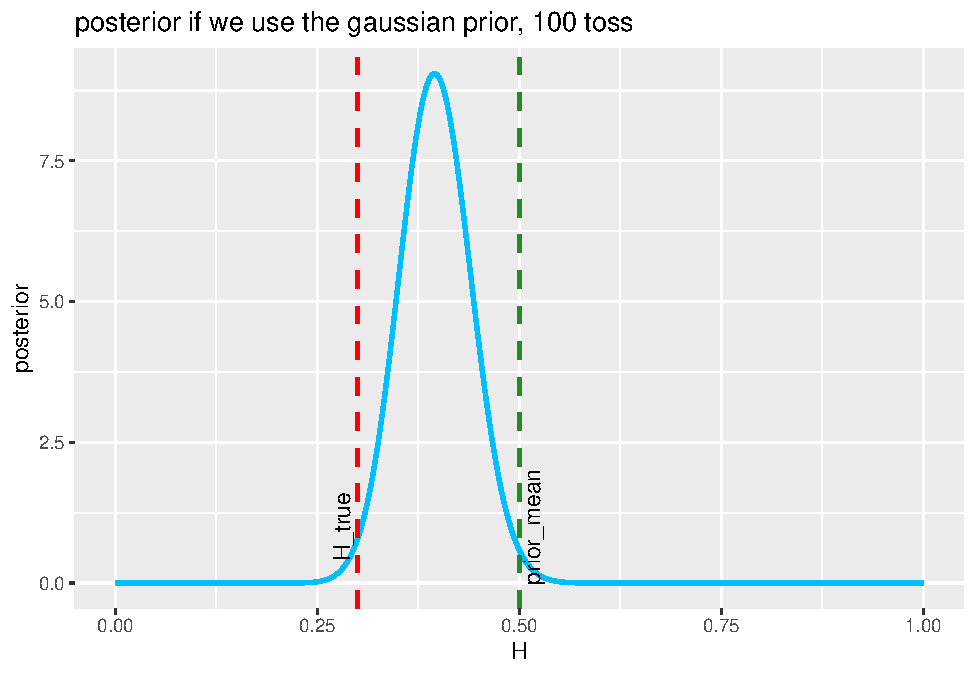
\includegraphics[width=0.75\linewidth]{astrostat-1_files/figure-latex/unnamed-chunk-13-1} \end{center}

\begin{center}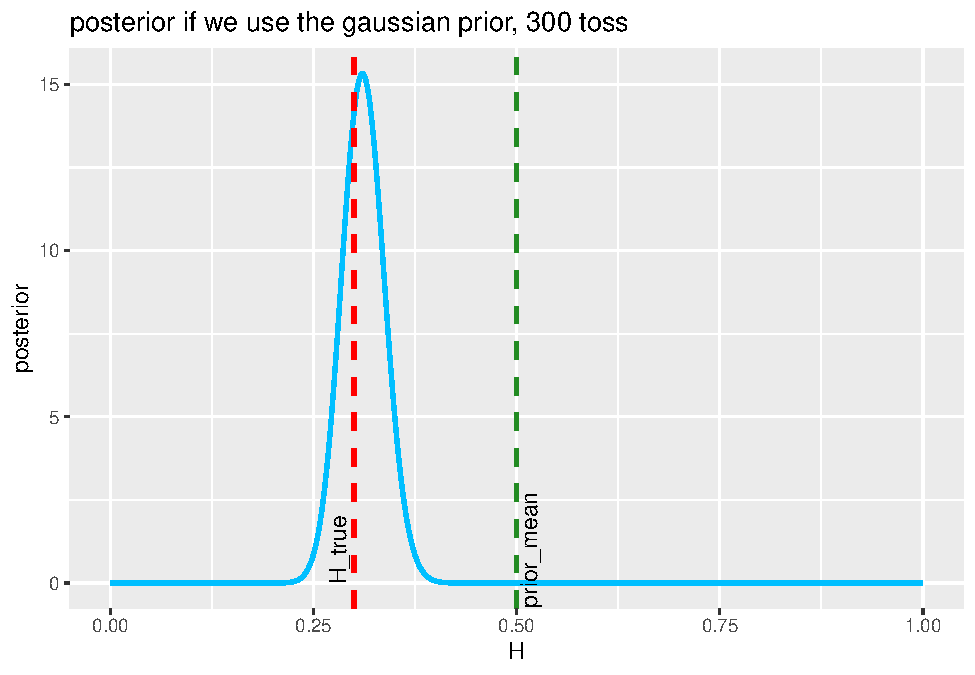
\includegraphics[width=0.75\linewidth]{astrostat-1_files/figure-latex/unnamed-chunk-14-1} \end{center}

\begin{center}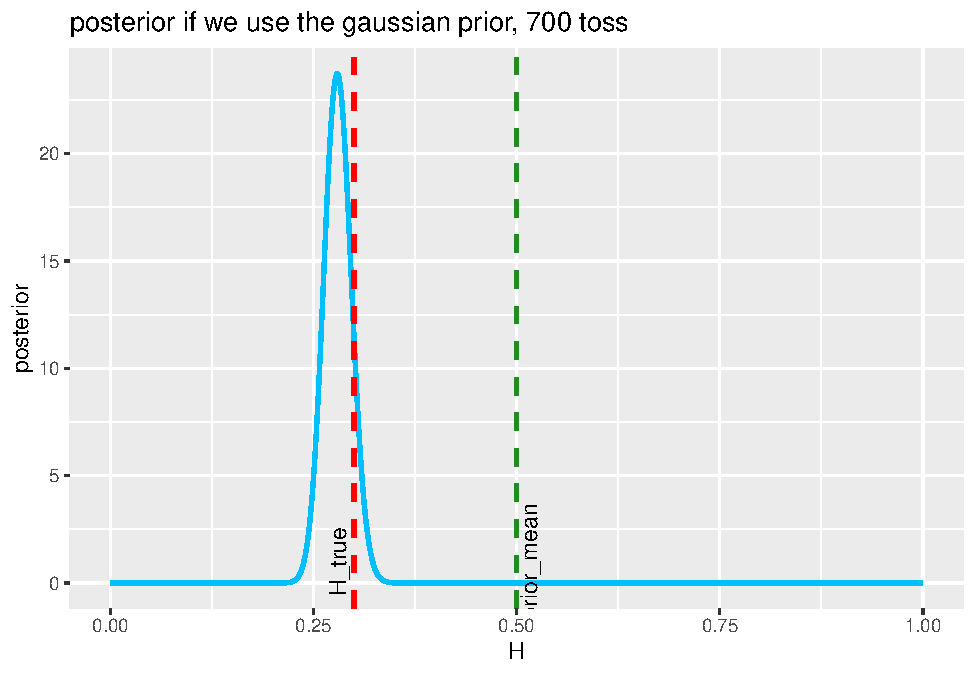
\includegraphics[width=0.75\linewidth]{astrostat-1_files/figure-latex/unnamed-chunk-15-1} \end{center}

\begin{center}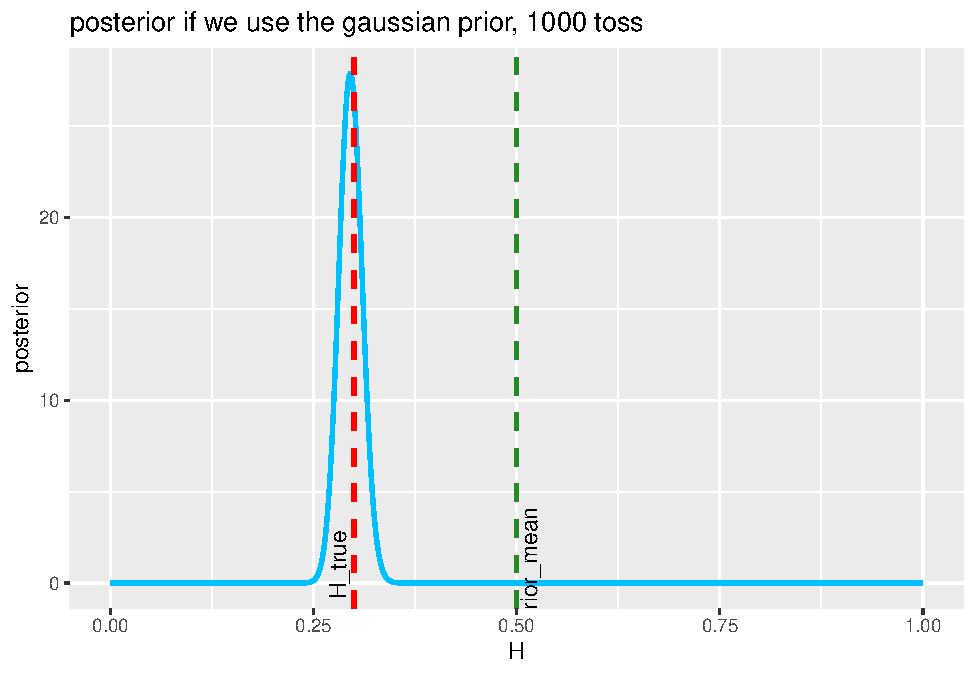
\includegraphics[width=0.75\linewidth]{astrostat-1_files/figure-latex/unnamed-chunk-16-1} \end{center}

\hypertarget{comparison-between-the-two-priors}{%
\section{Comparison between the two
priors}\label{comparison-between-the-two-priors}}

Having plotted both sequences of posteriors let's plot them together
side by side as a means of comparing them.

\begin{center}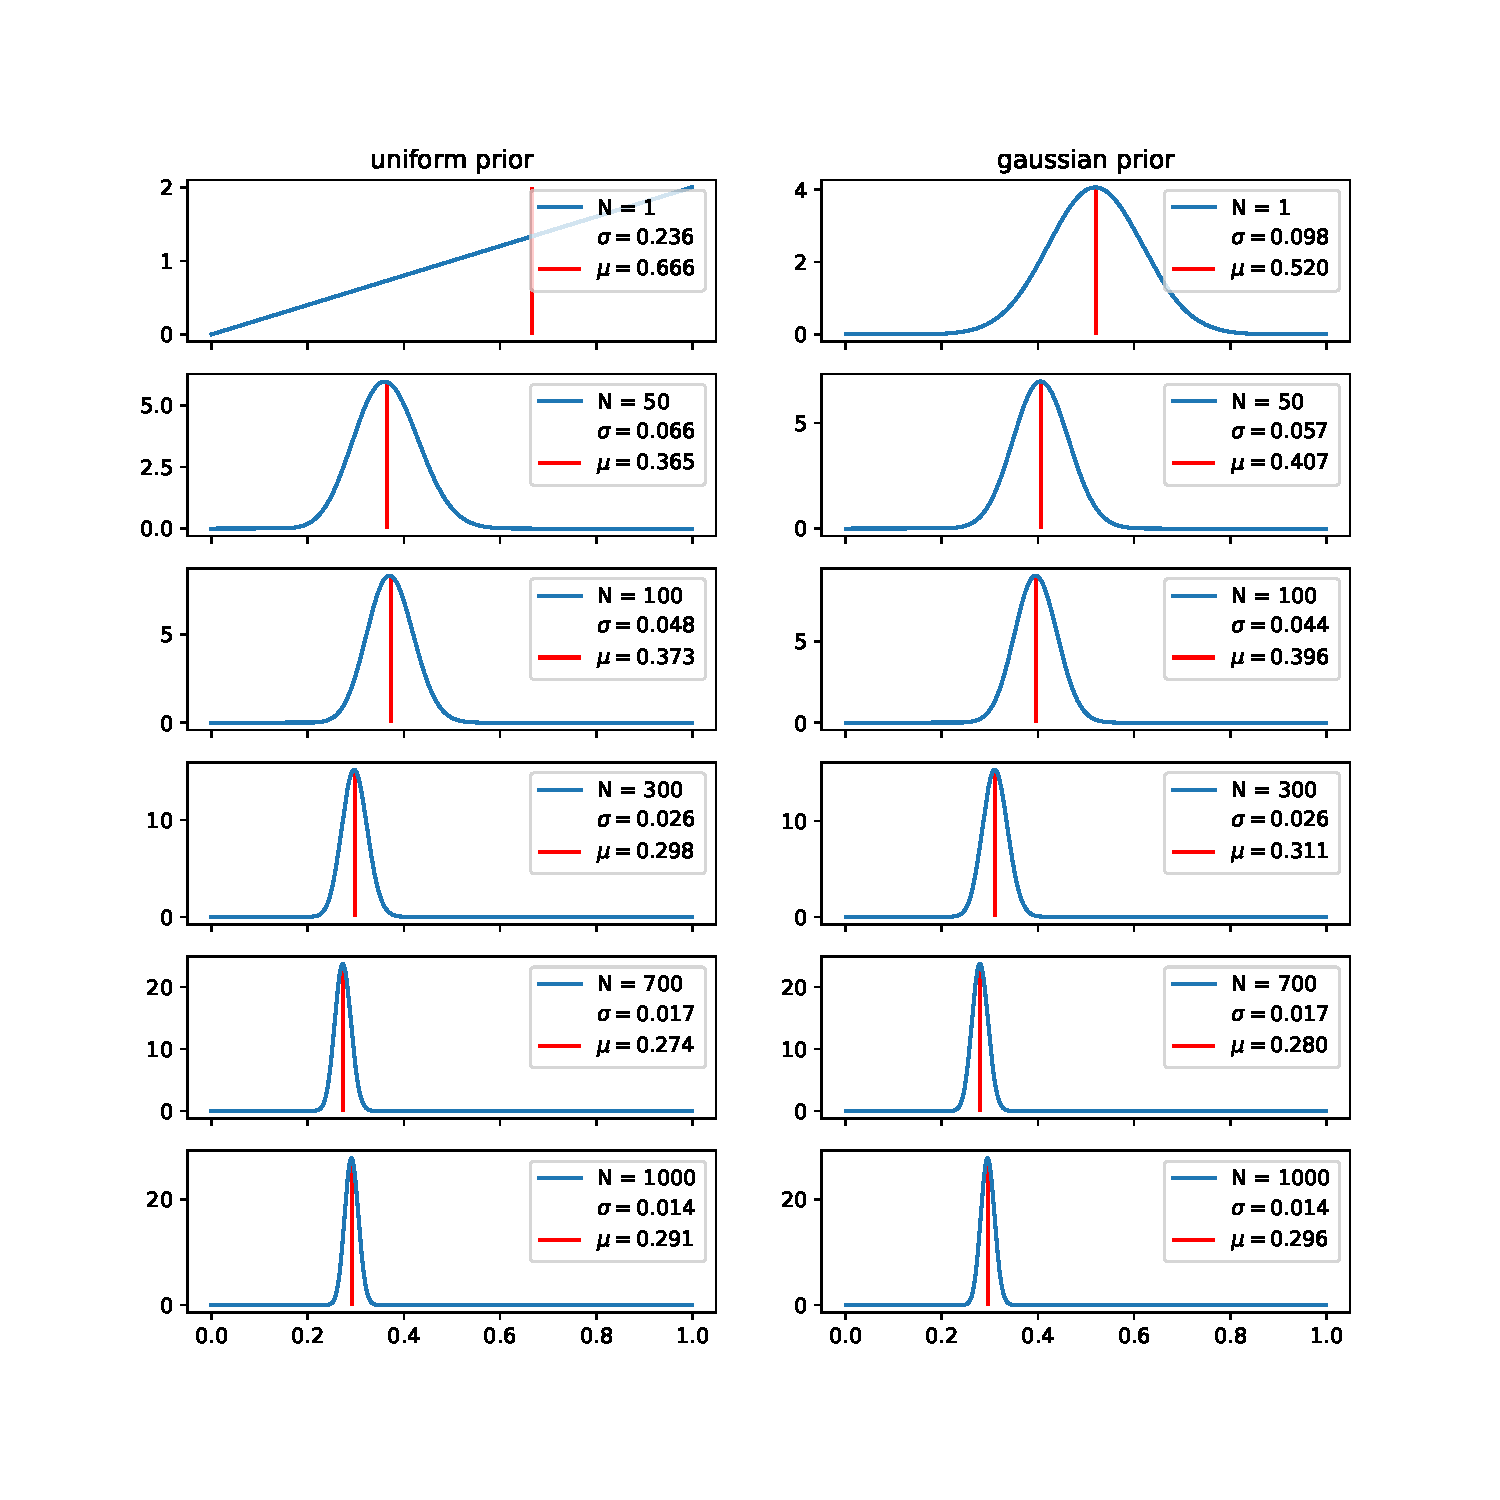
\includegraphics[width=1.0\linewidth]{./astrostat-1-comparison} \end{center}

The left column depicts the evolution of the posterior when we use the
uniform prior; similarly the right one contains the gaussian prior-based
posteriors. For each of these distribution the mean and variance values
(evaluated with a simple numerical scheme) are reported; this is useful
because the asymptotic distribution is guaranteed to be centered on 0.3
(the true value of \(H\)) with negligible variance \emph{irrespective of
the prior}.

We notice that if we use the uniform prior the posterior's mean
converges a bit faster, which is an intuitive result: an uniformative
prior immediately gives more importance to the data, whereas if we start
with a prior peaked around a wrong value for \(H\) we will need more
data to ``fix'' our distribution first. Therefore when we use the
gaussian prior the process of learning consists of moving the mean to
the left, then decreasing the width; with the other prior, instead, we
can get closer to the correct mean sooner. Of course this is only a
slight difference, since a lot of data is available almost immediately -
and therefore convergence to the asymptotic distribution is reached
easily in both cases.

\hypertarget{conclusion}{%
\section{Conclusion}\label{conclusion}}

We simulated a binomial process in order to study a simple but
significant example of Bayesian parameter inference. In particular we
were able to verify two important results, which are a general
consequence of known theoretical results:

\begin{itemize}
\item
  starting with a ``wrong'' prior slows down convergence because some
  data will be spent initially to ``fix'' the distribution, whereas
  starting with a prior which is closer to the asymptotic distribution
  (or at least more similar to it than the available alternatives)
  speeds up convergence. Indeed we expect that if we modified the
  gaussian prior so that the mean was much closer to \(H_{\text{true}}\)
  we would reach convergence even faster.
\item
  when the dataset is very large the likelihood dominates, in the sense
  that the final posterior is approximately insensitive to the chosen
  prior.
\end{itemize}

\end{document}
